\documentclass{article}
\usepackage{graphicx}
\begin{document}
\graphicspath{{fotos/}}
\section{Diseño y evolución de las clases principales del Modelo}
\subsection{Diseño del tablero}
Toda la lógica que implementa el concepto del tablero queda reflejada a lo largo de todo el proyecto en la clase Board.
\subsubsection{Sprint 1}
La clase Board es un simple contenedor de cubos, organizados en forma de matriz.
No tiene interacción con otros objetos del modelo.
\subsubsection{Sprint 2}
Ahora la clase Board tiene la funcionalidad de actualizarse a sí mismo una vez se coloca un nuevo cubo, funcionalidad que antes estaba delegada a la clase Game.
\subsubsection{Sprint 3}
A partir de este Sprint los tableros tienen forma (es decir, la forma no es necesariamente siempre cuadrada) y tamaño elegido por los usuarios. A parte, Board tiene una representación en forma de String y de JSONObject, a través de los métodos toString() y report().
\subsubsection{Sprint 5}
Ahora, aparte de guardarse los cubos del tablero en forma de matriz, se guardan en forma de lista por ser una representación de los datos muy conveniente en distintas partes del proyecto, entre otras, para la red.

\subsection{Diseño de los colores}

\subsection{Diseño de los cubos}

\subsection{Diseño del juego}
La clase fundamental del juego es la clase Game, la clase principal del modelo.
\subsubsection{Sprint 1}
La clase Game responde a ejecuciones del PlaceCubeCommand, colocando nuevos cubos en las casillas seleccionadas, actualizando el tablero, manejando los turnos de los jugadores y actualizando sus puntos.
\subsubsection{Sprint 2}
A partir de este momento, Game no se encarga de actualizar el tablero y las puntuaciones de los jugadores, sino de únicamente pasarle al tablero los cubos nuevos que tiene que insertar. El tablero, a partir de ese cubo, se actualiza a sí mismo, y los cambios de cubos actualizan las puntuaciones de los jugadores.
\subsubsection{Sprint 3}
Game tiene su propia representación en forma de String y de JSONObjet, a través de los métodos toString() y report().
\subsubsection{Sprint 4}
A partir de este sprint, Game pasa a ser una clase abstracta y se pasa a tener dos modos de juego, el clásico (jugadores individuales) y el modo por equipos, que son implementados por las clases herederas de Game: GameClassic y GameTeams.
También se implementa el patrón MVC, por lo que Game (modelo) pasa a tener una lista de observadores y métodos para el envío de notificaciones a estos.
\subsubsection{Sprint 5}
Game se adapta con ciertos cambios y nuevos métodos para soportar el juego en línea.
\subsubsection{Sprint 6}
En este momento Game sufre su mayor refactorización. Esta clase pasa a extender de la clase Thread, de forma que ya no funciona ejecutando comandos en el mismo momento de su creación, sino que estos de ponen en espera y Game, que está en todo momento funcionando y comprobando si hay nuevas peticiones puestas en espera, las ejecuta cuando puede. Esto nos permite evitar problemas de desbordamiento con el cálculo de jugadas por parte de las inteligencias artificiales, aparte de permitir el funcionamiento esperado de la vista sin comprometer su rendimiento.
Aparte, Game deja de llevar a cabo el manejo de turnos y se delega esa responsabilidad a la clase TurnManager, que es invocada tras cada jugada para que ejecute (si procede) el siguiente turno.

\subsection{Diseño de los jugadores}

\subsection{Diseño de los equipos}

\subsection{Diseño del gestor de turnos}

\subsection{Diseño de los estados del juego}

\subsection{Diseño de las replays}

\subsection{Diseño de las Inteligencias Artificiales}
\subsubsection{Sprint 5}
Las estrategias son externas al modelo. El cómputo de movimientos a través de estas estrategias de hace a partir de la vista, a través de la clase PlayerView, que representa al Player en la vista y se encarga de ejecutar sus acciones. Por razones de encapsulación, las estrategias no tienen acceso al modelo y realizan sus cálculos a través de GameStates.
\subsubsection{Sprint 6}
Las estrategias ahora forman parte del modelo, siendo atributo de aquellos Players controlados por la máquina. Como en este punto el manejo de turnos se lleva a cabo por la clase TurnManager y el modelo funciona en su propia hebra, la clase PlayerView desaparece del proyecto y son los propios players quienes ejecutan las estrategias, que a nivel abstracto resulta mucho más intuitivo. Por la hebra del modelo, cuando las estrategias terminan de calcular el siguiente movimiento, este no se ejecuta en ese mismo instante, sino que se deja en espera en el modelo hasta que este pueda ejecutarlo.


\section{Diseño del Controlador}


\section{Diseño de la Vista de GUI}

\subsection{Diseño del menú principal y pantallas pre-juego}

\subsection{Diseño de la pantalla de juego}


\section{Diseño de la Vista de Consola}

\subsection{Diseño del menú principal y pantallas pre-juego}

\subsection{Diseño de la pantalla de juego}


\section{Diseño de la red}

\subsection{Diseño del servidor}

\subsection{Diseño de los clientes}


\section{Diseño y evolución de las Historias de Usuario}

\subsection{Como usuario quiero que Rolit introduzca características innovadoras pensando en las posibilidades que brinda el multijugador: Inteligencias Artificiales}

\subsubsection{Sprint 5}
Este fue el Sprint en el que se empezaron a desarrollar las distintas estrategias de las inteligencias artificiales. Se planearon tres, recogidas en las siguiente clases, todas herederas de la clase abstracta Strategy: RandomStrategy, GreedyStrategy y MinimaxStrategy.

La idea de la estrategia es que, cuando le toque jugar a una inteligencia artificial, la estrategia se encarge de calcular
su siguiente movimiento y este se ejecutase inmediatamente después de su cálculo.

Para encapsular está lógica se creo la clase abstracta Strategy, para que cada estrategia en particular fuera una clase
heredera de esta.

Se han desarrollado tres estrategias, que suponen tres niveles de dificultad distintos, 
y la lógica de estas está recogida en las siguientes clases: RandomStrategy, GreedyStrategy y MinimaxStrategy.

\textbf{RandomStrategy}:
La idea es que se genere una posición cualquiera en el tablero, siempre y cuando esta sea válida. Esta es la posición que la inteligencia artificial jugará.
Lógicamente, la tendencia general las inteligencias artificiales que aplican esta estrategia es no obtener una gran cantidad de puntos, por lo que esta estrategia es la de nivel fácil.

\textbf{GreedyStrategy}:
Esta estrategia tiene por intención analizar el tablero en busca de la posición que le garantiza al jugador el máximo número de puntos en este mismo turno. Esta estrategia lleva a jugadas mucho mejores y elaboradas, pero sigue sin ser la mejor, así que representa el nivel de dificultad medio.

\textbf{MinimaxStrategy}:

Antes de explicar la implementación de esta estrategia en el caso de Rolit, debemos explicar primero en qué consiste la estrategia Minimax en teoría de juegos:

\textbf{Estrategia Minimax en teoría de juegos}: 

En teoría de juegos, el Minimax busca minimizar la pérdida esperada. La aproximación que se toma es asumir que el oponente va a tomar las decisiones que más te perjudiquen. De esta manera, al encontrar la decisión que menor pérdida suponga, el resultado real será siempre igual o mejor al calculado, de forma que el cálculo es fiable.

La mejor forma de explicar esto es a través de un ejemplo:

Imaginemos que estamos en un juego de dos jugadores, uno contra el otro, basado en turnos, en el cual ambos jugadores conocen en todo momento el estado actual de la partida en su totalidad. Un buen ejemplo de esto es el ajedrez. Supongamos pues que juegas con las piezas blancas, y tu adversario juega con las piezas negras. En cada uno de tus movimientos vas a jugar el movimiento que consideres que más te favorece. Por el otro lado, bajo nuestra aproximación, suponemos que el otro jugador va a jugar el movimiento que más te perjudique. Podemos hacer una representación de esto en forma de árbol:

Imaginemos que cada nodo contiene un número que representa el estado actual de la partida (para esto hace falta tener un criterio de valoración del estado actual de la partida, en el cual no entraremos en detalle en el caso del ajedrez, pero más adelante sí en el caso del Rolit), y cada arista representa un movimiento jugado, por el cuál se desciende en el árbol de un estado de la partida al siguiente. En cuanto a la valoración de los estados del juego, si el número de un nodo es positivo va ganando el jugador blanco (a mayor mejor); si el número es negativo, va ganando el jugador negro (a menor peor). Como el juego va por turnos, si un nivel del árbol se corresponde con el turno de un jugador, el siguiente nivel se corresponde con el siguiente jugador. De esta forma, volviendo al ejemplo propuesto, si desde un nodo se conoce el valor de todos sus descendientes pueden pasar dos cosas: si es el turno del jugador blanco, tomará la decisión que le lleve al mayor valor; si es el turno del jugador negro, tomará la decisión que le lleve al menor valor. 

Se ilustra el funcionamiento del algoritmo en la siguiente imagen: 

\begin{center}
\centering
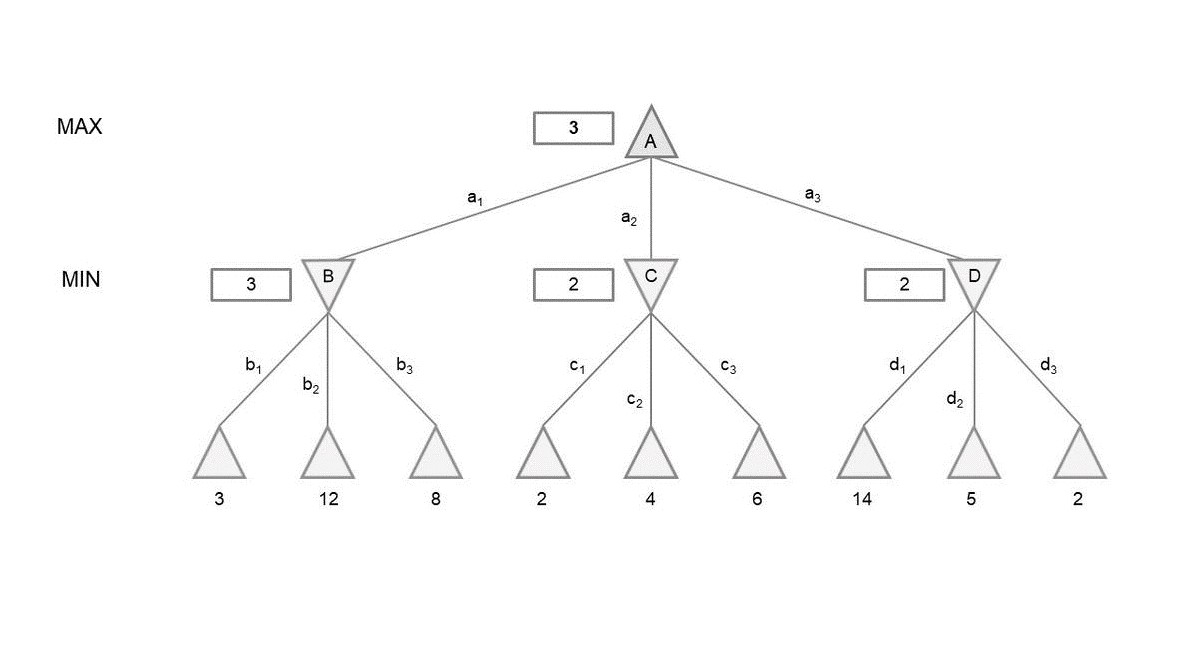
\includegraphics[scale=0.5]{minimaxExample.jpg}
\end{center}
%%FIXME Centrar

En el caso del ajedrez (y de la mayoría de juegos por turnos, como Rolit) hay siempre muchos posibles movimientos a jugar. De esta forma, en el árbol de decisión, de cada nodo salen muchos descendientes, resultando en un algoritmo con coste aproximadamente exponencial en el promedio de jugadas disponibles. Esto hace que la búsqueda del mejor posible movimiento se convierta en un problema intratable en no demasiados niveles de profundidad de búsqueda. Por tanto, surge la obligación de limitar la profundidad hasta la que se quiere hacer la búsqueda.

Volviendo ahora al Rolit, no estamos en un juego de dos jugadores (o al menos no necesariamente).
Afortunadamente, en este juego el criterio de valoración de jugadas es fácil: La mejor jugada es la que te lleve a acabar con el mayor número de puntos.

Ahora, como hay más de dos jugadores, para conseguir un cálculo de puntos fiable, el cálculo se lleva a cabo considerando que el jugador propietario de la estrategia quiere hacer aquella jugada que más puntos le otorgue a la larga, mientras que el resto de jugadores en sus turnos hacen la jugada que más puntos le quite al jugador propietario. De esta forma se calculan puntos para el jugador propietario situándonos en la situación más desfavorable posible, de forma que todo aquello que se calcule va a derivar siempre en un resultado igual o mejor al calculado, de forma que los resultados de los cálculos son fiables.

Debido a lo exhaustivos que resultan estos cálculos (y tras comprobación empírica simulando numerosas partidas) la estrategia MinimaxStrategy representa el nivel difícil de las inteligencias artificiales.

Ahora, antes de la explicación más técnica, observemos que la estrategia GreedyStrategy se puede implementar aplicando una MinimaxStrategy en la que solo se explora un nivel de profundidad, puesto que en este nivel se busca la jugada que más puntos garantice, y no se sigue buscando más allá. Por tanto, a nivel de clases, la clase GreedyStrategy es heredera de MinimaxStrategy, y el atributo de profundidad máxima pasa a valer 0.

Pasamos ahora a explicar la implementación de estas estrategias:

Para la simulación de movimientos pensamos originalmente en usar la clase Board para colocar cubos y evaluar resultados, pero no tardamos en darnos cuenta de que esto era inviable, puesto que los métodos de Board tienen una comunicación con otras clases que no deseeamos para esto, puesto que nosotros simplemente queremos hacer simulaciones, y no cambios reales.

Es por esto que fue necesario crear otra representación del tablero puramente funcional y adaptada a la simulación de movimientos, de donde surgió la siguiente clase:

\textbf{SimplifiedBoard}:

Esta clase consta de una matriz en la que almacena el color de los cubos del tablero real. Para disminuir costes y evitar tener que hacer copias del tablero tras cada movimiento simulado, se lleva una pila con los cambios que se realizan al simular un movimiento, de forma que cuando se quiere dejar el tablero en el estado previo a la simulación para realizar otra simulación, en vez de realizar una copia se revierten los cambios aplicados, lo cual resulta mucho menos costoso.

En SimplifiedBoard también se almacenan los puntos de los distintos jugadores, puesto que la idea es consultar los puntos después de simular cada movimiento.

Ahora, para calcular el mejor movimiento para ejecutar, en la clase de la estrategia se realiza un bucle en el que se recorren todas las posiciones del tablero, consultando si cada posición es válida o no, y en caso de dar con una posición válida, se simula ese movimiento.

Dentro de la simulación, en SimplfiedBoard, si la profunidad a explorar es mayor que 0, antes de revertir los cambios se vuelve a realizar el bucle de las posiciones, pero simulando esta vez para el siguiente jugador, y así hasta que la profundidad a explorar es 0. Hay que tener en cuenta que el jugador propietario de la estrategia busca maximizar sus puntos, mientras que el resto de jugadores buscan minimizarlos. Por tanto, en los bucles de recorrido de posiciones, la estrategia es conocedora de para qué jugador esta simulando el siguiente movimiento, de forma que si está simulando para el jugador propietario devolverá el resultado más favorable, y si está simulando para cualquier otro jugador devolverá el resultado más perjudicial posible para el propietario. De esta forma, se podrá conocer el resultado final realista de cada jugada posible, y así elegir la mejor jugada para el jugador propietario.

El cómputo del movimiento a jugar a través de la estrategia Minimax, llevado a cabo en el método calculateNextMove(), se ilustra en el siguiente diagrama:

\begin{center}
\centering
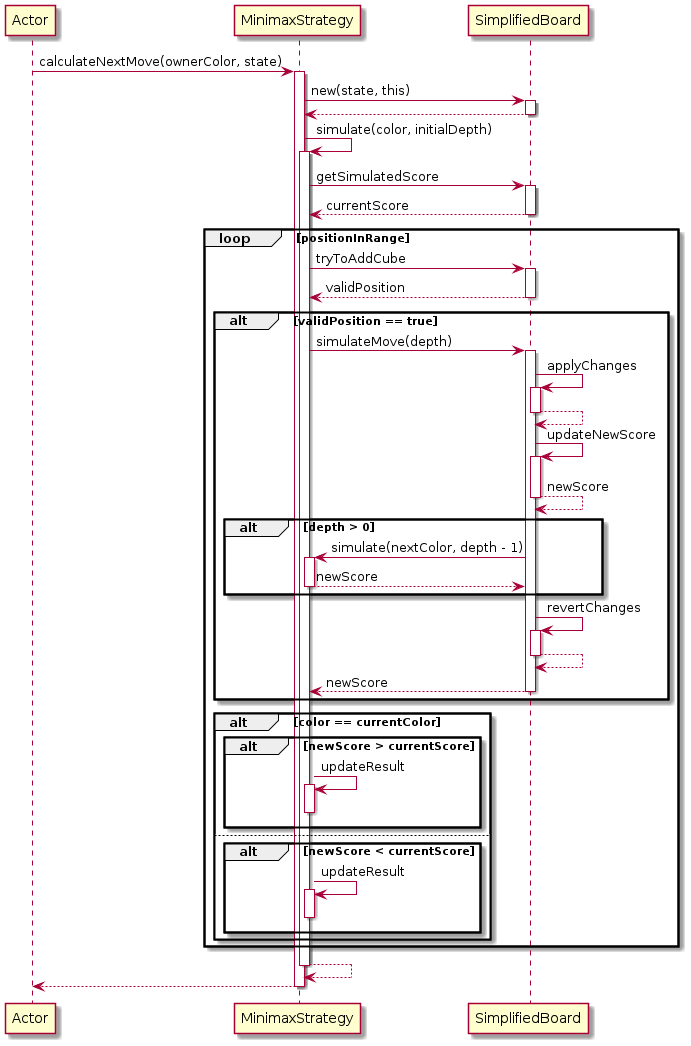
\includegraphics[scale=0.5]{Minimax.calculateNextMove()-Sprint5.png}
\end{center}

\subsubsection{Sprint 6}
Por motivos de eficiencia de MinimaxStrategy, se ha implementado de forma complementaria la poda alfa-beta, que se explica a continuación:

\textbf{Poda alfa-beta}:
La poda alfa-beta es una mejora del algoritmo Minimax. Se mantienen dos valores, alfa y beta, que representan respectivamente la puntuación mínima que se llevará el jugador maximizador y la puntuación máxima que se asegura el jugador minimizados. Inicialmente, alfa es $-\infty$ y beta es $\infty$. 

Siempre que la puntuación máxima que se asegura al jugador que minimiza se vuelve menor que la puntuación mínima que se asegura el jugador que maximiza se puede parar de explorar por la rama actual. De forma análoga, se podan ramas en el caso contrario.

La mejor forma de visualizar esta poda es a través de una ilustración:

\begin{center}
\centering
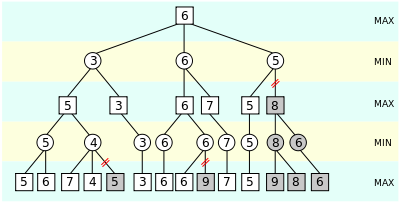
\includegraphics[scale=0.5]{poda alfa-beta.png}
\end{center}
%%FIXME Hacer más grande

Como vemos en este ejemplo, si exploramos en el árbol de izquierda a derecha, una verz llegamos a la rama derecha vemos que el jugador minimizador encuentra una rama por la que logra llegar al valor 5. Como minimiza, se sabe que el valor de ese nodo va a ser, como mucho, 5. Al ver esto el jugador maximizador, teniendo en cuenta que en una rama anterior ha llegado al valor 6, sabe que no tiene que seguir explorando esa rama, porque de ninguna manera va a encontrar un valor mejor que 6, y por tanto, en esta situación, el mejor resultado es el que le brinda empezar explorando la rama del centro.

Esta poda ha sido muy útil para reducir costes de cálculo, y el nuevo algoritmo mejorado queda reflejado en el siguiente diagrama:

\begin{center}
\centering
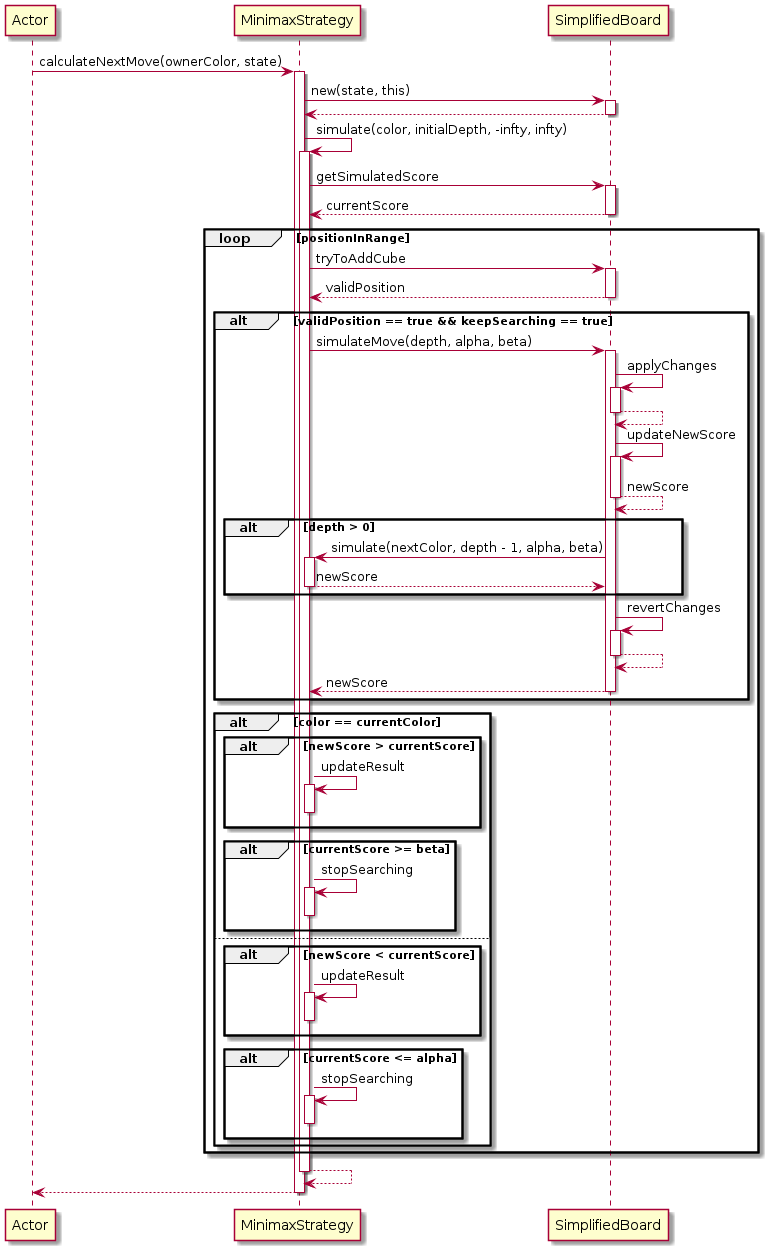
\includegraphics[scale=0.5]{Minimax.calculateNextMove()-Sprint6.png}
\end{center}

\end{document}